%% $RCSfile: proj_report_outline.tex,v $
%% $Revision: 1.3 $
%% $Date: 2016/06/10 03:41:54 $
%% $Author: kevin $

\documentclass[11pt
              , a4paper
              , twoside
              , openright
              ]{report}


\usepackage{float} % lets you have non-floating floats

\usepackage{url} % for typesetting urls

%
%  We don't want figures to float so we define
%
\newfloat{fig}{thp}{lof}[chapter]
\floatname{fig}{Figure}

%% These are standard LaTeX definitions for the document
%%                            
\title{The Title}
\author{The }

%% This file can be used for creating a wide range of reports
%%  across various Schools
%%
%% Set up some things, mostly for the front page, for your specific document
%
% Current options are:
% [ecs|msor|sms]          Which school you are in.
%                         (msor option retained for reproducing old data)
% [bschonscomp|mcompsci]  Which degree you are doing
%                          You can also specify any other degree by name
%                          (see below)
% [font|image]            Use a font or an image for the VUW logo
%                          The font option will only work on ECS systems
%
\usepackage[font,ecs]{vuwproject}

% You should specifiy your supervisor here with
%     \supervisor{Firstname Lastname}
% use \supervisors if there is more than one supervisor

% Unless you've used the bschonscomp or mcompsci
%  options above use
%   \otherdegree{OTHER DEGREE OR DIPLOMA NAME}
% here to specify degree
\otherdegree{Master of Artificial Intelligence}

% Comment this out if you want the date printed.
\date{}

\begin{document}

% Make the page numbering roman, until after the contents, etc.
\frontmatter

%%%%%%%%%%%%%%%%%%%%%%%%%%%%%%%%%%%%%%%%%%%%%%%%%%%%%%%

%%%%%%%%%%%%%%%%%%%%%%%%%%%%%%%%%%%%%%%%%%%%%%%%%%%%%%%

\begin{abstract}

A short description of the project goes here.

\end{abstract}

%%%%%%%%%%%%%%%%%%%%%%%%%%%%%%%%%%%%%%%%%%%%%%%%%%%%%%%

\maketitle

\chapter*{Acknowledgments}\label{C:ack} 
Any acknowledgments should go 
in here, between the title page and the table of contents.  The 
acknowledgments do not form a proper chapter, and so don't get a 
number or appear in the table of contents.

\tableofcontents

% we want a list of the figures we defined
\listof{fig}{Figures}

%%%%%%%%%%%%%%%%%%%%%%%%%%%%%%%%%%%%%%%%%%%%%%%%%%%%%%%

\mainmatter

%%%%%%%%%%%%%%%%%%%%%%%%%%%%%%%%%%%%%%%%%%%%%%%%%%%%%%%

% individual chapters included here
\chapter{Introduction}\label{C:intro}

\subsection{The reinforcement learning problem}

Reinforcement learning is a framework that describes how an agent learns by interacting with the environment. The framework involves 2 entities the agent and environment. The agent is the only entity that we as designers have direct control of. We decide how its learns and decides on its actions. The environment is the context and situation that the agent is in. There are three important flows of information;  the state of the environment to the agent, the action decision to the environment and lastly the reward to the agent. This can be best be understood in the figure below.

\begin{fig}
\begin{center}
    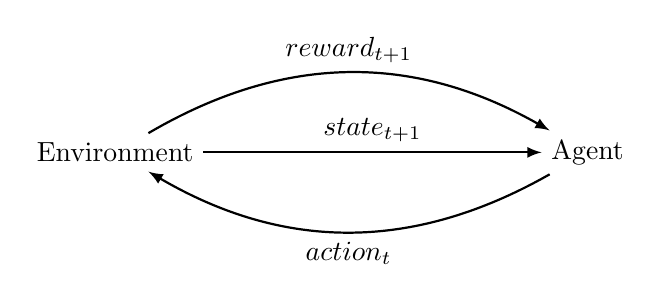
\begin{tikzpicture}[
        node distance=6cm, % Increased node distance for better spacing
    ]
        % Define nodes
        \node (env) {Environment};
        \node (agent) [right of=env] {Agent};

        % Define arrows and labels without boxes
        \draw [-latex,bend left, thick] (env) edge node[anchor=south] {$reward_{t+1}$} (agent);
        \draw [-latex, thick] (env) -- node[anchor=south] {$state_{t+1}$} (agent);
        \draw [-latex,bend left,thick] (agent) edge node[anchor=north] {$action_{t}$} (env);
    \end{tikzpicture}
    \caption{The flow of information between th environment and agent}
\end{center}
\end{fig}

The state is a representation of the information within the environment that the agent observes to make its decision on which action to take. The reward signal is treated as the final word on how good the previous state action was, the more reward the better, always. Lastly the action taken by the agent is sent to the environment and the environment will in turn return the next state and reward. This brings us to the reinforcement learning problem which can be framed as such "How does the agent decide which actions to take given the state such that it maximises the future cumulative reward". It is important that the agent maximises all \textit{future cumulative} reward otherwise short term gains could be made to the sacrifice of larger long term gains. This idea has been formalised by Richard Sutton as the reward hypothesis

\begin{quote}
    "That all of what we mean by goals and purposes can be well thought of as maximization of the expected value of the cumulative sum of a received scalar signal (reward)." 
    \cite{suttonReinforcementLearningSecond2018}
    \label{quote:reward}
\end{quote}

\subsection{Formalism}

The reinforcement problem can be formalised as a Markov Decision Process (MDP). The MDP is a collection of states, actions and rewards along with a transition function which states the probability of the next reward and state given a state and reward. This makes the MDP a 4-tuple $(S,\mathcal{A}, \mathcal{P}, R)$ where $S$ is the set of states, $\mathcal{A}(s)$ is the set of actions that can be taken from state $s$, $\mathcal{P}$ is the transition function and $R \subset \mathbb{R}$ is the set of rewards. The transition function is defined as:

\begin{equation}
\mathcal{P}(s',r, s,a) = Pr\left\{ S_{t}=s', R_{t}=r | S_{t-1}=s, A_{t-1}=a \right\}
\label{eq:transition}
\end{equation}
Where $s,s \in S, a \in \mathcal{A}(s) \text{ and } r \in R$.

This transition function completely characterises the dynamics of the environment. The abstraction of the environment to a MDP is widely applicable and serves as the basis for much of reinforcement learning. We can see here that transition function only looks at the previous state. It can do this because we assume that the state representation has the \textit{Markov property} \cite{suttonReinforcementLearningSecond2018}. The Markov property states that including previous states in the conditional wont change the probability of next state reward tuple. In other words $\mathcal{P}(s_{t+1}, r_{t+1}, s_{t},a_{t}) = \mathcal{P}(s_{t+1}, r_{t+1}, s_{t},a_{t}, s_{t-1}, s_{t-2}, ... , s_{0})$. Therefore a state with the Markov property is a sufficient representation of the history of the agent-environment interaction. In some problems the agent only partially observes the state meaning the Markov property is not satisfied. This is called a partially observable MDP (POMDP) and is a more complex problem to solve which wont be addressed in this report.

The agent interacts with the MDP to produce a trajectory of states, actions and rewards. Because the agent will not know the transition function \ref{eq:transition} it will have to learn about the MDP from the information in a trajectory \ref{eq:MDPsequence}.

\begin{equation}
S_{1},A_{1},R_{2},\dots S_{n},A_{n}, R_{n+1},\dots 
\label{eq:MDPsequence}
\end{equation}

In this trajectory \ref{eq:MDPsequence} we have an infinite sequence as this is an example from a continuing MDP that has no end. Alternatively you could have episodic MDPs that have a start and end with a terminal state. Episodic MDPs require practical considerations in implementing algorithms. However for most of the theory it make no difference as you can think of a episode MDP as a continuing MPD with a state that transitions to itself and gives reward 0.

"The cumulative sum of a received scalar signal" part of the reward hypothesis \ref{quote:reward} can be formalised to be the return $G$.

\begin{equation}
G_{t}=R_{t+1}+\gamma R_{t+2}+\gamma^{2}R_{t+3}\dots=\sum_{k=t}^{\infty}\gamma^{t-1}R_{t+1}
\end{equation}

$\gamma$ is called the discounting factor and weights future rewards to have less effect on the return. It is usually added for two reasons. Firstly because it makes the return finite which simplifies the mathematics. Secondly is due to the very natural intuition that the future is less predicable than the present, thus more distance rewards should have less weight as they are less certain. 


A agent will use policy $\pi$ which provides the probability of taking action $a$ given state $s$. This policy could be deterministic or stochastic.
To evaluate how good a policy is or how much reward we can expect at a state we need a function to tell us. This is called the value function and it is a expectation of the future rewards.

\begin{equation}
v_{\pi}(s)=\mathbb{E}\left[ G_{t}| S_{t}=s\right] 
\end{equation}

The state value function depends on the state, policy and discounting factor $\gamma$ which is used by the return. In a similar vain to the state value function we have the action-value function which is the expected future reward given a state and action taken.

\begin{equation}
q_{\pi}(s,a) = \mathbb{E}\left[ G_{t} | S_{t}=s, A_{t}=a \right] 
\end{equation}

We can understand how to compute the expectation of the value function by looking at the Bellman equation \cite{suttonReinforcementLearningSecond2018}. The Bellman equation is based off the notion that the value of a situation should be the immediate reward you get plus the value of the situation you end up in. This can be written for the state value function as follows:

\begin{equation}
v_{\pi}(s)=\sum_{a}\pi(a|s)\sum_{s',r}p(s',r|s,a)\left[ r+\gamma v_{\pi}(s') \right]
\end{equation}
$\pi(a|s)$ is the probability of taking action $a$ given state $s$ and $p(s',r|s,a)$ is the transition function. This equation can be solved for $v_{\pi}$ by iterating over all states and actions until the value function converges. This is called the iterative policy evaluation and is a dynamic programming technique \cite{bellmanDynamicProgramming1957}.

The maximising part of the reinforcement problem can be solved by the finding optimal actions. We can define both $v_{\star}=\underset{ \pi }{ \text{max} }\ v_{\pi}(s)$ and $q_{\star}=\underset{ \pi }{ \text{max} }\ q_{\pi}(s,a)$ as the optimal value given optimal actions afterwards.
If we can find $q_{\star}$ then the problem is solved as we could make a policy $\pi_{\star}$ that is greedy with respect to $q_{\star}$. Two things stop this from being so simple. Firstly is that in many real problems we don't know the true transition function, therefore we either have to learn/approximate or learn the value/policies in a way that doesn't involve the transition function. Secondly is the computational complexity of iterating over all states and actions as well as all possible policies. This is called the curse of dimensionality and is a major problem in reinforcement learning. If we try to learn and transition funtion and come up with a model of the environment then we are using model based methods, alternatively we ignore the model and learn the value or policy directly and these are called model free methods. In the rest of the report we will be focusing on model free methods.

The form of explicitly learning a value function then implicitly getting actions from it is called value based methods. Alternatively you can learn the policy directly with policy based methods. The effectiveness of these methods depend heavily on how easy the value function or policy is to learn.
%% $RCSfile: using.tex,v $
%% $Revision: 1.1 $
%% $Date: 2010/04/23 01:57:05 $
%% $Author: kevin $
%%
\chapter{Using this document and the \texttt{vuwproject} style}\label{C:us}

If you are writing an MSc or PhD thesis you should \emph{not} be using this style. Instead use \verb=vuwthesis=, which is based on the book style, and conforms to the VUW thesis rules. The thesis style is rather different from the project report style. 

This document is formatted using a local (to ECS and MSOR at VUW) style file. When you write your project report you should be very careful when changing the beginning. The document class settings should read:

\begin{verbatim}
\documentclass[11pt
              , a4paper
              , twoside
              , openright
              ]{report}
\end{verbatim}
The options to the document class specify that:
\begin{itemize}
\item 11pt font is to be used for the main body text,
\item  we will print on A4 paper, 
\item we will use duplex (two-sided) printing,
\item we want chapters to start on a right-hand page. 
\end{itemize}

The opitons you supply to the  \texttt{vuwproject} style will depend upon
what you are using the style for.

\subsection{Specifying the details}
The \texttt{vuwproject} style sets up the front page properly, and provides various commands allowing you to specify the author, title, supervisor or supervisors, the school from which the report is being submitted and the degree that the report is being submitted for. The style has deliberately been designed to do as little as possible. This means that your document can easily be re-formatted as a technical report, or for submission to a conference or journal by using the appropriate style.

It is also possible to use the style to easily produce documents on a
stand-alone computer where your \LaTeX installtion might not have all
of the  files and fonts available to machines within ECS or MSOR.

Most of the options to the \texttt{vuwproject} style are currently a simple
choice and there's a default that will make it obvious if you do not make
a choice.

Use one of the following options to use fonts available on ECS/MSOR machines
or to use images that imitate them (assumes you have copies of the images)
\begin{itemize}
\item \verb+font+
\item \verb+image+
\end{itemize}

Use one of the following options to set the school,
\begin{itemize}
\item \verb+ecs+
\item \verb+msor+
\end{itemize}

Use one of the following options to choose a pre-defined degree,
\begin{itemize}
\item \verb+bschonscomp+
\item \verb+mcompsci+
\end{itemize}

or use this command to use an explicit degree or diploma name
\begin{itemize}
\item \verb+\otherdegree{DEGREE OR DIPLOMA NAME}+
\end{itemize}

So, for example, to submit a report for the Master of Comp Sci degree, which
the style knows about, from within ECS, using the images, you'ld ensure the
 \texttt{vuwproject} line options looked like:

\begin{verbatim}
\usepackage[image,ecs,mcompsci]{vuwproject}
\end{verbatim}

whereas for a degree from within MSOR, when creating the final version on
an ECS or MSOR machine where you have access to the fonts, you would use
these options

\begin{verbatim}
\usepackage[font,msor]{vuwproject}
\end{verbatim}


and add the other degree's name using this command 

\begin{verbatim}
\otherdegree{DEGREE OR DIPLOMA NAME}
\end{verbatim}

To specify the supervisor or supervisors use either of the following commands in the preamble.
\begin{itemize}
\item \verb+\supervisor{The Supervisor}+
\item \verb+\supervisors{Super 1 and Super 2}+
\end{itemize}

If you fail to set any degree or supervisor, or the school, then the front page will report this.

The \texttt{vuwproject} style also sets the default font to be Palatino, using the \texttt{mathpazo} package. Palatino is one of VUW's `offical' fonts, and is the font used for the heading on the front page. The \texttt{mathpazo} package also typesets maths in a style which suits Palatino. 

\section{Copying the style}
If you want to write your project report away from VUW you will need to make your own copy of the \texttt{vuwproject} style.

You can find out where the original lives by reading the messages that \LaTeX\ prints when it is run.

Alternatively, you can down load a copy of the  \texttt{vuwproject} style from
the ECS webpages.

Any changes made to your own copy of the \texttt{vuwproject} style will not be reflected in the original, and \textit{vice versa}. Hence it makes sense to leave this as it is, and use a local style file for your own definitions.   

\chapter{Some \LaTeX\ hints and tips}\label{C:ex}
\LaTeX\ is a very good tool for producing well-structured documents 
carefully. It is very bad tool for banging things together in a rush 
and panic. 

\section{Floats}
One perennial problem with \LaTeX\ is its treatment of 
\emph{floats}.  Suppose you have a figure or table which you want to 
include in your document. Where should it go? Traditional typesetting 
practice is to put these in some convenient place, such as the top or 
bottom of the current or next page, or at the end of the section or 
chapter.  \LaTeX\ adopts a similar strategy, and allows floats to 
``float'' away from where they were defined. You can give a hint 
about where you want the figure, but \LaTeX\ may move it. Sometimes 
this is fine but sometimes you may want to have more control and 
insist that a float goes \emph{here}. Anselm Lingau's 
\textsf{float} package gives you this flexibility. For example, the following figure is an example of a non-floating float:

\begin{fig}[H]
\begin{center}
\begin{tabular}{l|lll}
$\delta$ & $\mathit{a}$ & $\mathit{b}$ & $\Lambda$ \\ \hline 
$S_{1}$  & $\{\}$       & $\{\}$      & $\{S_{2}, S_{5}, S_{10}\}$\\
$S_{2}$  & $\{S_{3}\}$  & $\{\}$      & $\{\}$\\
$S_{3}$  & $\{S_{4}\}$  & $\{\}$      & $\{\}$\\
$S_{4}$  & $\{S_{3}\}$  & $\{\}$      & $\{\}$\\
$S_{5}$  & $\{\}$       & $\{S_{6}\}$ & $\{\}$\\
$S_{6}$  & $\{\}$       & $\{S_{7}\}$ & $\{S_{8}\}$\\
$S_{7}$  & $\{S_{6}\}$  & $\{\}$      & $\{\}$\\
$S_{8}$  & $\{S_{9}\}$  & $\{\}$      & $\{\}$\\
$S_{9}$  & $\{\}$       & $\{S_{8}\}$ & $\{\}$\\
$S_{10}$ & $\{S_{11}\}$ & $\{\}$      & $\{\}$\\
$S_{11}$ & $\{\}$       & $\{S_{10}\}$& $\{\}$\\ 
\end{tabular}
\caption{The transition function of an NFA with $\Lambda$  transitions}

\end{center}
\end{fig}

On the other hand, Figure \ref{Fig:two} is a floating float. 



\begin{fig}[tbh]
\begin{center}
\begin{tabular}{l|ll}
$\delta''$ & $\mathit{a}$ & $\mathit{b}$ \\ \hline 
$T_{1}$  & $T_{2}$ & $T_{3}$\\ 
$T_{2}$  & $T_{4}$ & $T_{5}$\\ 
$T_{3}$  & $T_{6}$ & $T_{7}$\\ 
$T_{4}$  & $T_{8}$ & \\
$T_{5}$  & $T_{10}$ & \\
$T_{6}$  &  & $T_{11}$\\ 
$T_{7}$  & $T_{3}$ & \\
$T_{8}$  & $T_{4}$ & \\
$T_{10}$  &  & $T_{5}$\\ 
$T_{11}$  & $T_{6}$ & 
\end{tabular}
\caption{The transition function of an FA to accept 
the same language.}
\label{Fig:two}
\end{center}
\end{fig}

You can define different types of new floats, and you can have tables 
of them in the contents pages.


\section{URL's}
Use \verb=\url= from the \textsf{url} package to typeset URL's. Just 
using \verb+\texttt+ or \verb+\tt+ does not work:

\begin{itemize}
\item \verb+\texttt{http://www.mcs.vuw.ac.nz/~neil/}+
\item \verb+\url{http://www.mcs.vuw.ac.nz/~neil/}+
\end{itemize}

Give:
\begin{itemize}
\item \texttt{http://www.mcs.vuw.ac.nz/~neil/}
\item \url{http://www.mcs.vuw.ac.nz/~neil/}
\end{itemize}
If you use the \textsf{hyperref} package then you can produce PDF 
files with clickable hyperlinks using \verb=\url=.

\section{Graphics and \LaTeX}
\LaTeX\ offers rather poor support for the inclusion of graphics. 
There are lots of ways to include pictorial material in \LaTeX, all 
of which are deficient in some way or other. Look at \cite{GRM97GC} for a 
description of them. If your document does need to have pictures in it 
it is worth thinking about what is needed \emph{before} you generate 
the pictures.

\section{The bibliography}

You should build up your bibliography as you go along.  Trying to get 
the details of the bibliography correct at the end of the project is 
hard work. Make sure that you record all the relevant details. Beware 
that material on the internet is likely to change very rapidly. If you 
are going to include material which is only available on the internet, 
then you should probably include in the reference the date on which 
you obtained the document.

\section{Run \LaTeX, run}

\LaTeX\ builds up information about your document for the table of 
contents, references and so on at each run. This means that, for 
example, the table 
of contents is really the table of contents of the previous 
compilation. You may need to run \LaTeX\ two or three times to let it 
catch up with itself. If you have cross references within your 
bibliography (for example two papers from the same collection, such 
as \cite{Dum93a,Dum93b}) you may need to run 
BibTeX more than once. 

It is also possible that the table of contents file has garbage in 
it, and will prevent the document from being compiled. This may 
happen if you have had to abort compilation, due to a bug in the 
source file. If this is the case then removing the \texttt{.toc} file 
will usually solve the problem. You will have to fix the original 
bug, of course.


\section{Find out more by\ldots}
You can find out more by:
\begin{itemize}
\item reading any one of a number of books, such as \cite{GMS94,Lam94}. The 
VUW library has copies of these;
\item visiting  the Comprehensive \TeX\ Archive Network (CTAN) at 
\url{www.ctan.org};
\item typing \texttt{latex} into Google.
\end{itemize}

It is \emph{highly unlikely} that you are the first person who ever 
wanted to do what you want to do with \LaTeX. Therefore it is likely 
that someone has already solved your problem: the real key to using  
\LaTeX\ well is to make effective use of what other people have done.

\section{Summary}
In this chapter we explained some things about \LaTeX.
\chapter{Conclusions}\label{C:con}
The conclusions are presented in this Chapter.



%%%%%%%%%%%%%%%%%%%%%%%%%%%%%%%%%%%%%%%%%%%%%%%%%%%%%%%

\backmatter

%%%%%%%%%%%%%%%%%%%%%%%%%%%%%%%%%%%%%%%%%%%%%%%%%%%%%%%


%\bibliographystyle{ieeetr}
\bibliographystyle{acm}
\bibliography{sample}


\end{document}
